\documentclass[12pt, titlepage]{article}
\usepackage[french]{babel}
\usepackage[utf8]{inputenc}
\usepackage{fullpage}
\usepackage{setspace}
\usepackage{graphicx}
\usepackage{subfigure}
\usepackage{setspace}
\usepackage{tabularx}
\usepackage{hyperref}
\usepackage{times}
\usepackage{textcomp}
\usepackage{float}
\usepackage{capt-of}
\usepackage[toc,page]{appendix} 
\usepackage{lipsum}
\usepackage{booktabs}
\usepackage{enumitem}
\setlength{\parskip}{0.2cm}
\linespread{1.3}


% Taken from	tex.stackexchange.com/questions/88414/how-can-i-create-a-question-answer-format-for-reports
\newenvironment{QandA}{\begin{enumerate}[label=\bfseries\alph*.]\bfseries}
                      {\end{enumerate}}
\newenvironment{answered}{\par\normalfont}{}
\graphicspath{ {captures/} }
% % % % % % % Début des commandes % % % % % %
	\newcommand{\Poly}{École Polytechnique de Montréal}
	\newcommand{\SigleCours}{INF8500}
	\newcommand{\NomCours}{Systèmes embarqués: Conception et vérification}
	

        \newcommand{\uwriter}{Uart\_Write }
        \newcommand{\udriver}{Uart\_Driver }
        \newcommand{\ureceiver}{Uart\_Receiver }
        \newcommand{\ucheck}{Uart\_Check }
        \newcommand{\uconfig}{Uart\_Config }
        \newcommand{\urxtx}{Uart\_Rxtx }
        \newcommand{\theDut}{Uart DUT }
        \newcommand{\ucom}{Uart commerical }
        \newcommand{\refToStep}[2]{\hyperref[#1]{Étape \ref{#1}: #2}}
        \newcommand{\mss}{millisecondes }
        \newcommand{\cvp}{\emph{coverpoint }}                \newcommand{\cvg}{\emph{covergroup }}	
% % % % % % % Fin des commandes % % % % % %

\title{\Poly \\ \SigleCours --- \NomCours\\ \emph{TP1} }
\author{
\begin{tabular}
{l r}
Emilio Rivera & 1689355 \\ 
Théophile Gindre & 1864282 \\
Clément Gamache & 1642792 \\
\end{tabular}
\\ \\ \\ \\}
	\hypersetup{
		colorlinks,
		citecolor=black,
		filecolor=black,
		linkcolor=black,
		urlcolor=black
	}

\begin{document}
	\maketitle
        \begin{singlespacing}
	  \tableofcontents
        \end{singlespacing}
        \newpage
        \section{Analyse du DUT}
    	% Estimation des paramètres
	%\begin{figure}[H]
	%  \centering
	%  \includegraphics[width = \textwidth]{estimationParametre.png}
	%  \caption{Estimation des paramètres $\mu$ et $\sigma$ du taux d'homicide}
	%  \label{Estimation Parametre}
	%\end{figure}
	% Fin de l'estimation des paramètres
        
        Afin de démontrer le comportement de \emph{loopback} entre les broches d'envoi et de réception du UART, divisons le processus d'envoi de données en plusieurs étapes :
        \begin{enumerate}
          \item \label{rxtx:firststep} \udriver : Écriture de la donnée dans le registre TX  de \theDut. Cette écriture est présentée à la Figure 2 où les registres we et ce sont mis à 1 pour que la valeur en dat soit écrite à l'adresse de adr.
          \item \label{rxtx:secondstep} \theDut : Écriture en série sur TX et réception sur RX (branchement direct entre les deux ports entrée/sortie). Ce branchement est montré par la Figure 3.
          \item \label{rxtx:thirdstep}\udriver : Lecture de la valeur dans le registre RX. Cette lecture est présentée à la Figure 4 où we est mis à 0 et ce à 1 pour que la valeur en mémoire à adr soit "écrite" dans le registre dat.
        \end{enumerate}
        Il est montré explicitement à la Figure 1 que les signaux RX et TX suivent en tout temps les mêmes valeurs.
        
	    \begin{figure}[h]
	    	\centering
		    \caption{Mise en évidence de la relation entre le fil RX et TX}
	    	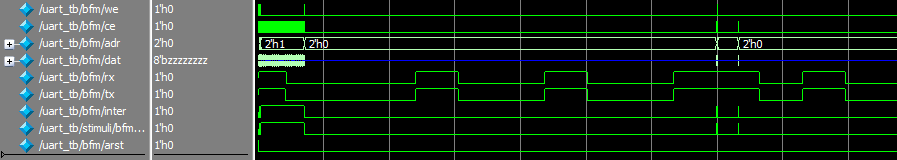
\includegraphics[ width= \textwidth]{rxIsTx.png}
    		\label{rxtx:rxtxscreenshot}
	    \end{figure}

		 \begin{figure}[h]
			\centering
			\caption{\refToStep{rxtx:firststep}{Écriture de la valeur 9 par \udriver dans le TX buffer}}
			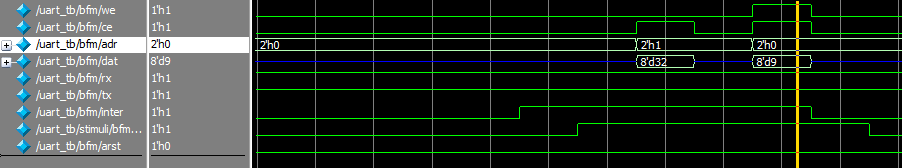
\includegraphics[ width= \textwidth]{write9.png}
			\label{rxtx:firststepscreenshot}
		\end{figure}
	
		\begin{figure}[h]
			\centering
			\caption{\refToStep{rxtx:secondstep}{Transmission sérielle par \theDut vers \udriver}}
			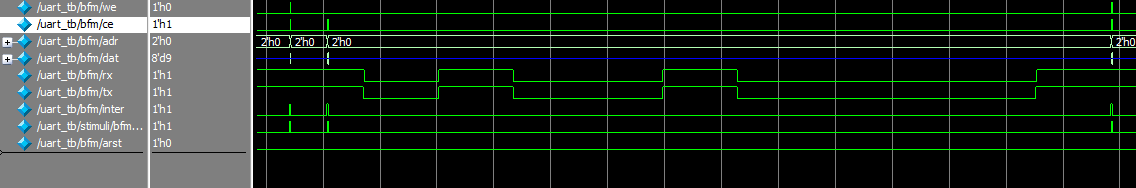
\includegraphics[ width= \textwidth]{serial9.png}
			\label{rxtx:secondscreenshot}
		\end{figure}
	
		\begin{figure}[h]
			\centering
			\caption{\refToStep{rxtx:thirdstep}{Lecture de la valeur 9 par \udriver dans le RX buffer}}
			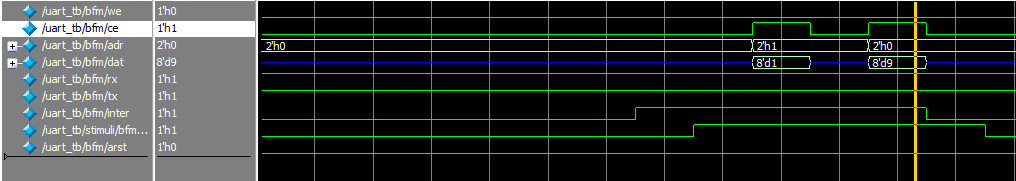
\includegraphics[ width= \textwidth]{read9.png}
			\label{rxtx:thirdstepscreenshot}
		\end{figure}

\section{Modification du DUT pour plan de test}
    \subsection{Test de transmission}
        Nous avons commencé par créer la classe \ureceiver afin qu'elle s'occupe de la lecture dans le RX buffer du \theDut et qu'elle place ensuite la valeur lue dans la mailbox "recept" destinée au scoreboard \ucheck. Nous avons alors rencontré un problème de synchronisation entre \udriver et \ureceiver. En effet, ces deux programmes étaient en attente d'une interruption sur le même Uart. Or ce modèle d'Uart ne possède qu'un seul fil d'interruption, qui est utilisé pour tous les types d'erreurs ou d'événements (la même interruption est créée lorsque le RX buffer est plein et lorsque le TX buffer est vide). 

	Prenons par exemple le cas où une donnée est disponible dans le RX buffer. Il est alors possible que le programme \udriver se réveille par l'interruption créée, alors que c'est \ureceiver qui aurait dû se réveiller pour traiter la donnée. 
    
    Pour résoudre ce problème, nous avons tenté de synchroniser les deux programmes grâce à un sémaphore, mais nous nous sommes rendus compte que l'utilisation de deux Uarts dans la suite du TP résolvait le problème. Pour la création du deuxième Uart, nous avons dupliqué le code d'implémentation du premier Uart et nous avons modifié la classe rxtx afin qu'elle connecte  le port TX de l'\theDut vers le port RX de l'\ucom. Après plusieurs tests, nous avons validé le fonctionnement de notre banc de test en accord avec la Figure 5 de l'énoncé.
    
    \subsection{Test de réception}
        Pour ajouter le test de réception au testbench, il nous a fallu connecter le port TX de l'\ucom au port RX de l'\theDut. Le même problème que pour la partie précédente a alors été rencontré, étant donné que les deux programmes \udriver et \ureceiver écoutent maintenant les interruptions des deux Uarts. Pour résoudre les conflits engendrés, nous avons utilisé un sémaphore de synchronisation entre \udriver et \ureceiver : le driver est mis en attente du sémaphore tant que le receiver n'a pas traité la précédente donnée envoyée. Ainsi, les deux programmes n'écoutent jamais les interruptions du même Uart simultanément. 
        
        Nous avons également adopté une convention pour le type de test effectué (test de l'envoi ou test de la réception). C'est le générateur (\uwriter) qui choisit aléatoirement un sens d'envoi des données et il transmet ce sens ainsi que la donnée à envoyer au \udriver à travers une seule mailbox nommée "envoi" (les deux messages sont placés dans la mailbox l'un à la suite de l'autre). L'\udriver lit alors en premier le sens, puis la donnée à envoyer. C'est ensuite à lui d'informer l'\ureceiver du sens choisi. Une mailbox "mailbox\_method" est utilisée pour cela. Une fois l'\ureceiver averti, l'\udriver peut alors placer la donnée sur le TX buffer du bon Uart (en fonction du sens sélectionné) et l'\ureceiver peut attendre une interruption sur l'autre Uart.


\section{Amélioration de la génération aléatoire} 
    \subsection{Création de la classe \uconfig} 
    La création de la classe \uconfig a été facile. La création de l'objet dans le programme de test est possible à partir de la méthode new(). Cette méthode initialise par défaut les valeurs des membres de la classe (qui sont décrits dans la prochaine section).

    Une subtilité à prendre en compte, qui est expliquée dans la documentation de SystemVerilog, est la façon dont il faut déclarer les membres de la classe de configuration. En effet, afin que l'appel à randomize() change effectivement la valeur des attributs, il faut que ces derniers soient définis comme rand ; le type des attributs doit être précédé par "rand".
    
    \subsection{Contenu de la classe \uconfig}
    Des membres de type enum ont été ajoutés dans la classe de configuration. Un comportement intéressant de la fonction randomize() appliquée sur des variables de type enum est le fait qu'une valeur aléatoire est choisie parmi les valeurs possibles de la structure. Ainsi, randomize() utilisé sur un enum avec quatre possibilités applique toujours une de ces quatre possibilités.
    
    \subsection{Modification de l'initialisation des modules} 
    Lors d'un changement de configuration, il fallait modifier l'initialisation des deux Uarts. Nous avons décidé que \udriver s'occuperait de l'initialisation des deux modules (DUT et commercial) pour plus de clarté. Dans la fonction d'initialisation de \udriver, un objet de la classe \uconfig est passé en paramètre. Concernant la configuration de la parité, Un simple décalage binaire de trois (afin d'écrire dans le troisième bit [il s'agit du bit de configuration de la parité]) suffit. Il ne faut pas oublier de mettre à 1 les deux premiers bits qui permettent la création d'interruptions.

    
    \subsection{Modification du programme de test}
    Dans le code initial, une seule génération de configuration était faite. C'est-à-dire que le testbench finissait quand l'un des modules avait terminé son exécution. Afin de changer la configuration régulièrement, nous avons choisi d'englober le tout dans un block repeat. Bien entendu, les configurations étaient changées à chaque itération à l'aide de randomize(). Le changement était ensuite appliqué grâce à l'appel de la fonction d'initialisation de \udriver.

	Après avoir fait cette modification, un autre problème survint : les temps d'exécution de chaque boucle étaient considérablement longs. En effet, dans le code précédent, \uwriter attendait 200 ms avant de terminer. Nous avons donc réduit cette valeur à 20 ms. 

    Par la suite, des problèmes de synchronisation furent détectées. Après avoir analysé les sorties sur la console des différentes valeurs testées dans les mailboxs, il nous apparut que lorsqu'une boucle du repeat était terminée, les mailbox n'étaient pas vidées. Par exemple, pour la deuxième configuration testée, la première valeur lue par \ucheck correspondait à la dernière donnée envoyée par \udriver dans l'itération précédente. À premier regard, le fait de vider les mailbox serait suffisant, mais cela ne permettrait pas à \ucheck de recevoir les dernières données envoyées (c'est d'ailleurs la raison de l'existence de l'attente de 200 ms dans le code original). Il fut donc déterminé qu'il fallait attendre que \ucheck ait reçu toutes les données envoyées avant de passer à l'itération suivante. Un fork avec une attente complète (fork / join) a donc été imbriqué dans le programme de test sur \uwriter et \ucheck. Ainsi, ces deux programmes doivent se terminer avant de passer à l'itération suivante (\udriver et \ureceiver s'exécutent à l'infini de leur côté). 


    \subsection{Vérification du changement de parité} 
		\begin{figure}[h]
			\centering
			\caption{Mise en évidence de la parité}
			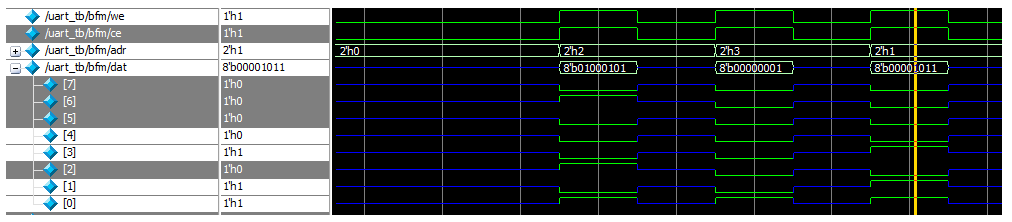
\includegraphics[ width= \textwidth]{parity.png}
			\label{random:parity}
		\end{figure}
        
        La figure 5 montre que l'\theDut vient de recevoir la valeur 11 (0b1011) et qu'il s'apprête à l'écrire sur TX. Lorsqu'on regarde la trace d'onde correspondant à l'envoi de cette valeur en série, on remarque que le bit de parité est à 1 (dans cet exemple, la parité est activée et est en mode \emph{ODD}, ce qui signifie que le bit de parité est à 1 si la valeur envoyée est impaire.
        
    \subsection{Mécanisme de génération aléatoire}
    a) En effet, il a été remarqué qu'à travers les multiples simulations, les mêmes valeurs apparaissaient. Il s'agit d'un mécanisme très intéressant dans le cadre de la vérification car les mêmes ensembles de données sont utilisées : si un problème est détecté dans l'un des ensembles, il est possible de relancer la simulation et d'obtenir exactement le même problème pour le même ensemble. Si les données étaient réellement aléatoires, obtenir de nouveau le problème serait une question de chance. Ceci facilite énormément le travail des personnes qui font la vérification, car reproduire le problème est parfois un long trajet.

    b) Il est possible de le faire en changeant la graine du simulateur (qui détermine la graine des modules) :

    \texttt{sim switch -sv\_seed [value]}
    
    c) Même si le testbench change, les valeurs aléatoires restent les même. En effet, ce n'est pas la compilation qui change la génération de nombre : il s'agit de la graine de génération. Cette graine est spécifique à la simulation. Comme précédemment expliqué, il s'agit d'une très bonne fonctionnalité car elle assure la reproductibilité de la simulation. Il est par ailleurs possible de changer cette grain entre les simulations.
    
    % http://www.doulos.com/knowhow/sysverilog/SNUG13_random_stability/SNUG2013_SV_Random_Stability_paper.pdf


\section{Injection d'erreurs} 
	
	La plus grande difficulté que nous avons rencontrée pour cette étape fût la synchronisation entre les bits pour l'injection d'erreur (c'est à dire le temps d'attente entre l'envoi de deux bits consécutifs sur le fil RX du \theDut). Ce temps d'attente correspond normalement au baudrate de l'Uart de transmission, mais en utilisant cette valeur, nous obtenions des retards ou des avances.
	
	Il a ensuite été décidé de vérifier la validité de notre valeur en regardant la \emph{waveform} obtenue sans injection d'erreur. Suite à l'observation de cette dernière, nous avons vu que la valeur calculée théoriquement était peu éloignée (à $ \pm5 \%$). Des tentatives de calcul furent effectuées afin de découvrir comment la valeur exacte devait être obtenue, mais en vain. Les valeurs finales furent donc extraites manuellement depuis les \emph{waveform} (puis confirmées par un email un peu plus tard).
    
	C'est la classe \urxtx qui s'occupe d'injecter l'erreur. Pour cela, elle intercepte les données qui transitent de \ucom vers \theDut et elle injecte l'erreur au bon endroit en fonction du type d'erreur souhaité. C'est \udriver qui envoie le type d'erreur à \urxtx à travers une mailbox appelée "err\_rxtx".
    
    \emph{Remarque} : Nous avons décidé de ne pas synchroniser l'injection d'erreur avec le scoreboard \ucheck, car nous n'avons pas jugé nécessaire que le scoreboard soit averti du type d'erreur (une simple vérification de la différence des valeurs envoyées et reçues suffit).
    
    \subsection{Injection du Parity Error} 
    	Il s'agit du bit indiquant la parité du message : chaque transmission complète est constituée de 11 bits dans lesquels 8 constituent le message, 2 démarquent le début et la fin et 1 indique la parité du message. Ainsi, en changeant le bit de parité (le neuvième à passer dans le fil dans chaque transmission), et si le bit de parité est activé, l'\theDut devrait être en mesure de détecter l'erreur.
    	    	
    \subsection{Injection du Framing Error} 
    	Il s'agit simplement de créer un décalage dans la transmission vers \theDut. Pour faire cela, nous avons utilisé l'instruction \emph{wait} lors de la transmission de l'un des bits (peu importe lequel). De ce fait, tous les bits suivants seront décalés.

    \subsection{Injection du Data Error} 
    	Ici, il s'agit simplement d'inverser un bit dans le message envoyé à \theDut. C'est \udriver qui génère le numéro du bit à inverser et qui l'envoie à \urxtx grâce à la mailbox "err\_rxtx".


\section{Couverture}
    \subsection{Couverture du baudrate et des types d'erreur} 
    	Un premier \cvg a été créé dans la classe de configuration. Nous avons laissé Questa générer les \emph{bins} automatiquement pour le \emph{baudrate} et pour le type d'erreur (car SV crée automatiquement les bins correspondant aux valeurs possibles dans le cas d'une variable de type enum). Par la suite, un coverpoint de type \emph{cross} a été utilisé pour générer un produit cartésien des bins de baudrate et d'erreur. Cela résulte en $4 * 5 = 20$ possibilités. 
		
    \subsection{Couverture de la détection d'erreur} 
		Pour avoir un \cvg qui comptabilise les erreurs détectées par les modules Uarts, nous avons supprimé le \cvg de \udriver et nous l'avons placé dans \ureceiver. Nous avons utilisé deux coverpoints : un pour chaque Uart. Les deux coverpoints sont échantillonnés à partir de deux variables "status" utilisées pour lire les registres de statut des deux Uarts. Enfin, \ureceiver appelle \emph{cg.sample()} à chaque donnée reçue, ce qui a pour effet de mettre à jour le \cvg avec les données du registre de statut (et notamment les erreurs détectées).

		Nous remarquons tout d'abord que l'\ucom ne détecte aucune erreur. Cela est normal, car nous n'injectons que des erreurs à destination de l'\theDut. Concernant les erreurs détectées par l'\theDut, on remarque que la relation n'est pas parfaite. 
        
        Dans le cas d'une erreur de parité, cela est dû au fait qu'elle peut être causée par les trois types d'erreurs injectées : un changement du bit de parité entraînera bien sûr une erreur sur la parité ; une \emph{Data error} cause aussi une erreur sur la parité puisque le fait d'inverser un nombre impair de bits rend le bit de parité incorrect ; enfin, une injection d'erreur sur le \emph{framing} pourrait causer une erreur sur la parité : un bit serait sauté dans le message et causerait possiblement une erreur sur le message, ce qui pourrait influencer la parité du message. De plus, les erreurs de parité ne sont pas prises en compte si la parité est désactivée. Toutes ces raisons font que le nombre d'erreurs de parité détectées ne correspond pas exactement au nombre d'erreurs de parité injectées. 
        
        De leur côté, les \emph{Data error} ne sont pas détectées et les \emph{Overflow error} ne sont pas gérées par notre programme. Enfin, les \emph{Framing error} correspondent quasiment au erreurs injectées (le nombre diffère de quelques unités, pour une raison que nous n'arrivons pas à expliquer).
		
    \subsection{Automatisation de la fin de test} 
    	 Le programme de test a été modifié en conséquence afin conduire les tests jusqu'à ce qu'une couverture complète du \cvg de \uconfig soit effectuée (toutes les couples [erreur, baudrate] ont été testés). Ainsi, la configuration est générée aléatoirement puis un test est fait, le tout tant que la couverture est inférieure à 100\%.
		
		Dans un cas idéal, nous aurions besoin de 20 itérations afin de tester entièrement le \cvg en question. Dans notre cas, 59 itérations furent nécessaires avant d'obtenir une couverture complète.
        
    	Remarque : il suffit d'utiliser la fonction \emph{get\_inst\_cov} afin d'obtenir la couverture courante et d'utiliser un compteur d'itération afin de limiter la boucle du programme de test à un nombre maximum.
    	
    	 \begin{table}[h!]
			 	\begin{center}
			 		\caption{Itérations nécessaires en fonction de la couverture désirée}
			 		\label{tab:cvgit}
			 		\begin{tabular}{c|c}
			 			Couverture (\%) & Itérations nécessaires\\
			 			\midrule
						   100   & 59 \\
                           75   & 10 \\
			 		\end{tabular}
			 	\end{center}
		 \end{table}
    	
\section{Assertions}
  \subsection{Ajout de l'assertion}
Une assertion doit être positionnée à un endroit critique, où l'erreur que nous désirons détecter a la plus forte chance de l'être. Pour cette raison, nous avons choisi de placer l'assertion associée à la condition donnée juste avant une lecture de \ureceiver.

Nous aurions également pu nous exercer en lançant une assertion sous la condition que le bit de partié ne concorde pas avec les données reçues. Cette assertion aurait également pu être envoyée tout juste avant une lecture de \ureceiver parce que ce moment précis possède une vue sur tous les états de l'Uart suite à ce qu'un cycle soit complété.

\section{Questions pour les améliorations du testbench}
	1)

	2)

\end{document} 
